\chapter{Other Factors}
\label{sec:otherfactors}

So far, we have examined anchor placement as the sole factor impacting localization error.  We set out here to show that there are indeed other factors that play a significant role in determining localization performance.

In the following example, the same anchor set is used in four different random networks.  Figure~\ref{fig:AS6good} shows two non-outlier cases.  The mean error for each network, despite using the same anchor set, is different.  What is surprising is the degree to which they are different: 37\%.  Figure~\ref{fig:AS6bad} shows two more networks with the same anchor set.  This time, both of the plots reveal outlier cases.  Despite using the same anchor set, the localization performance differs significantly.  While we have shown that anchor placement does play a role in the localization performance, these simple examples clearly show that there are significant other factors affecting the localization error.

\begin{figure}
  \centering
	\subfloat[Network A]{\label{fig:AS6NetworkDiff7}
		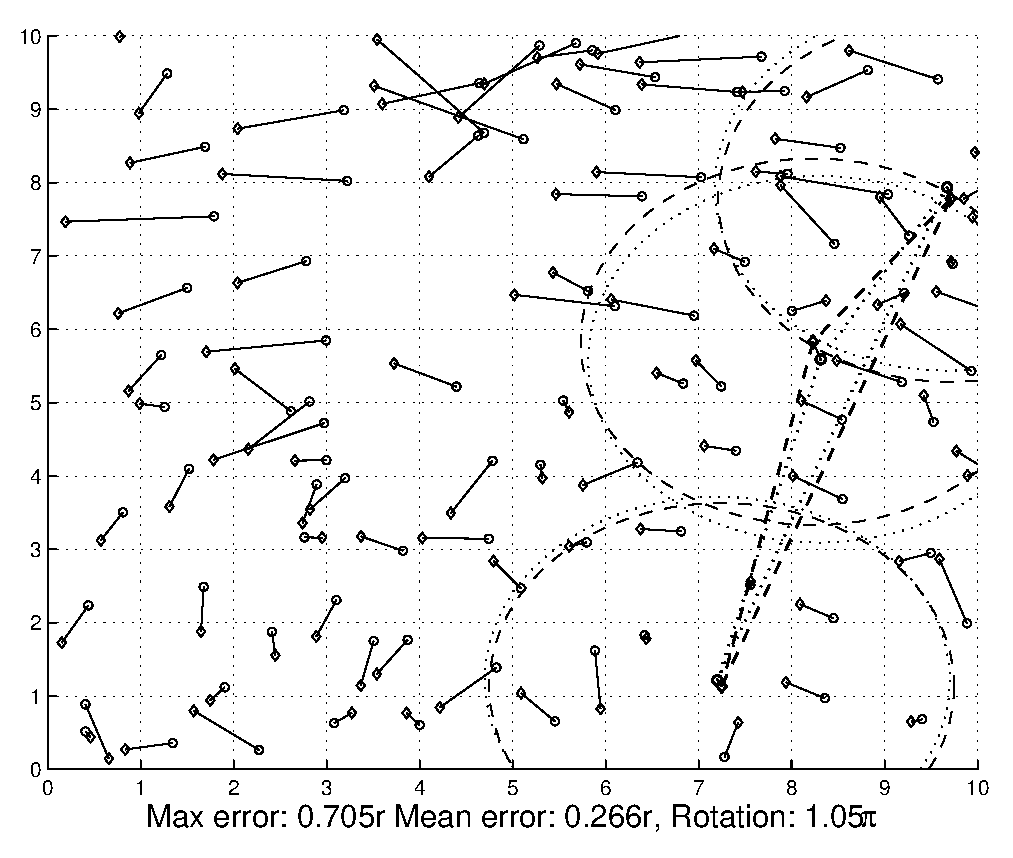
\includegraphics[width=\figurewidth\textwidth]{outliers/AS6/AS6NetworkDiff7}}
	\\
	\subfloat[Network B]{\label{fig:AS6NetworkDiff10}
		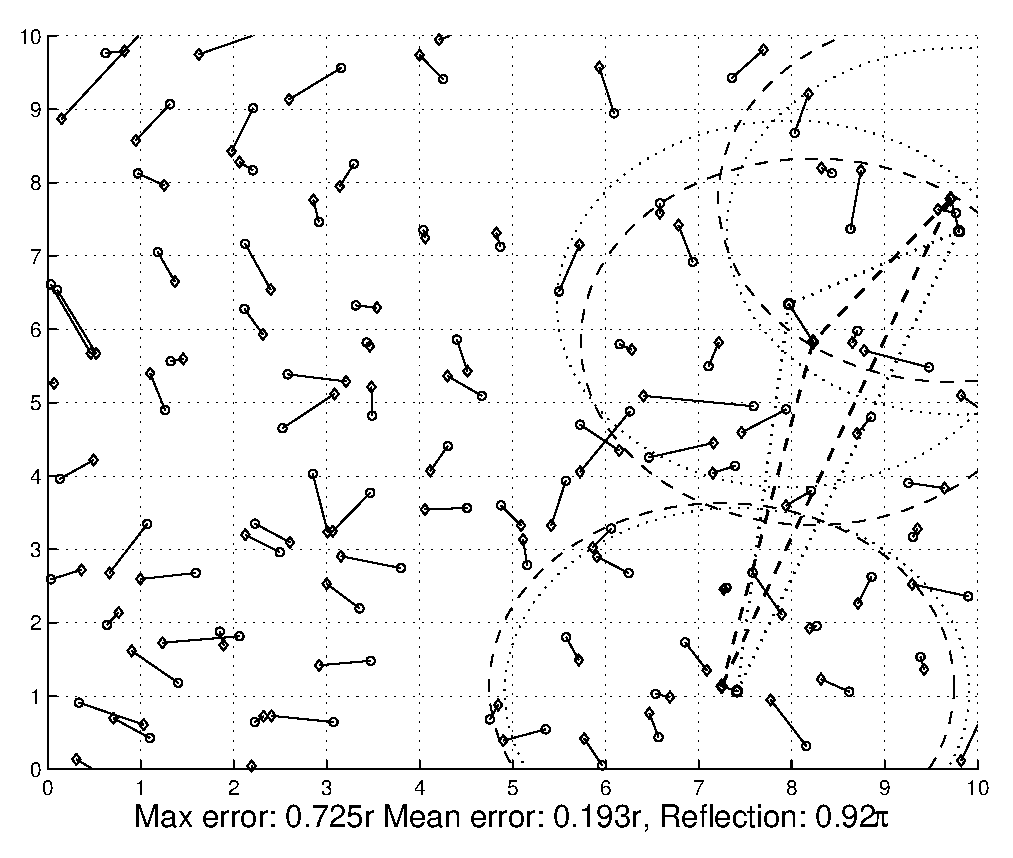
\includegraphics[width=\figurewidth\textwidth]{outliers/AS6/AS6NetworkDiff10}}
	\caption{Good localization performance with same anchor set in two different networks}
	\label{fig:AS6good}
\end{figure}

\begin{figure}
  \centering
	\subfloat[Network C]{\label{fig:AS6NetworkDiff9}
		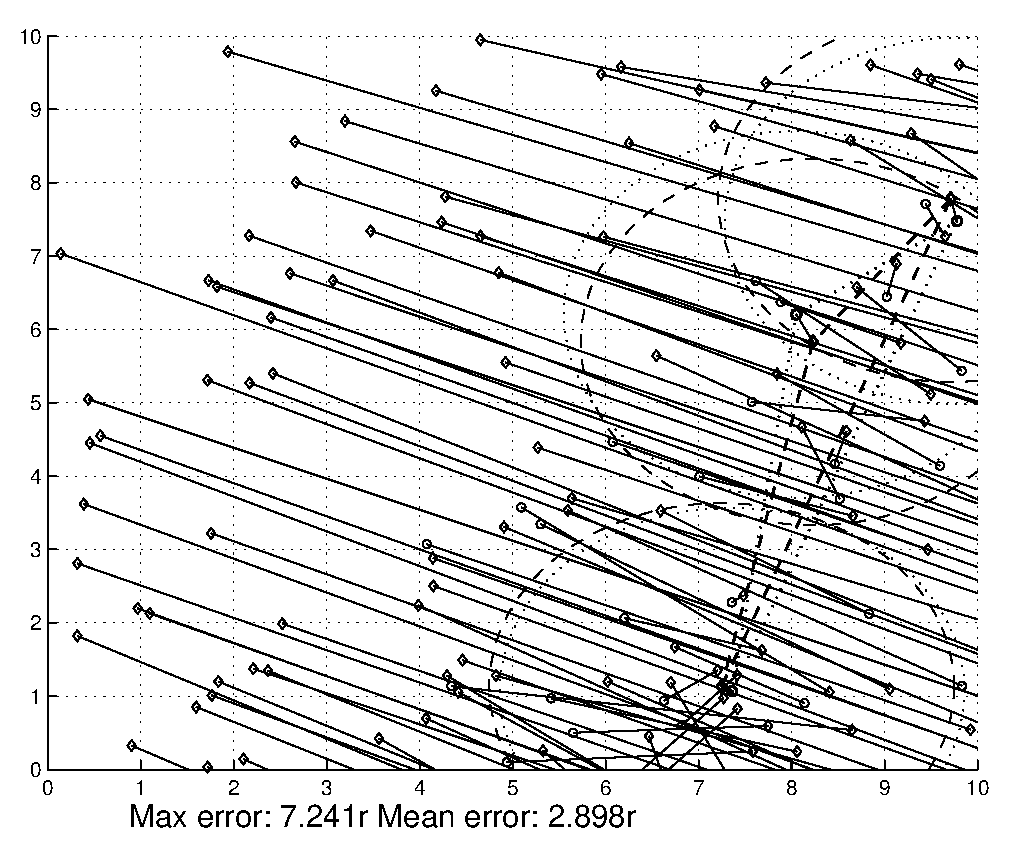
\includegraphics[width=\figurewidth\textwidth]{outliers/AS6/AS6NetworkDiff9}}
\\
	\subfloat[Network D]{\label{fig:AS6NetworkDiff8}
		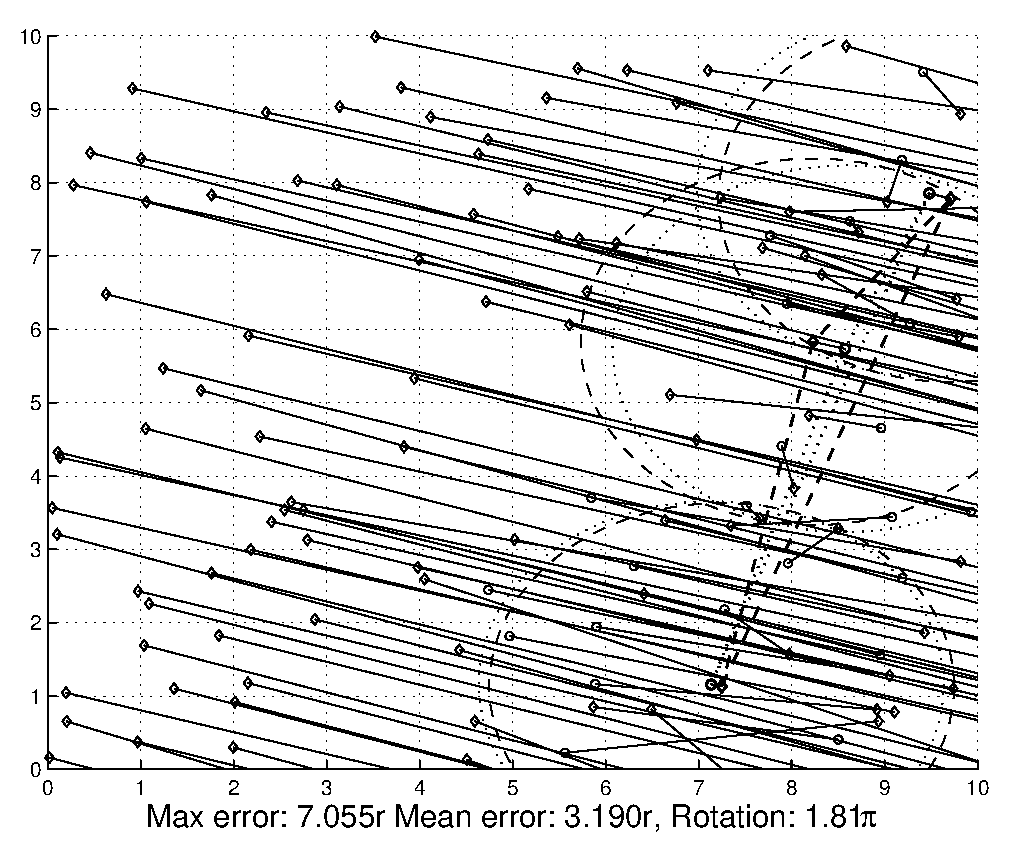
\includegraphics[width=\figurewidth\textwidth]{outliers/AS6/AS6NetworkDiff8}}	
    \caption{Poor localization performance with same anchor set in two different networks}
	\label{fig:AS6bad}
\end{figure}

These results show that there is significant variation in localization results across networks, when the anchor set is geographically fixed.  In other words, the absolute anchor positions are not enough to predict localization errors.  Therefore, it is clear there are other factors besides anchor placement effecting the resulting location errors. A key piece of future work is to isolate and analyze these other factors.  However, since the outlier case itself is undetectable in the absence of extensive ground truth data, the best we can hope for is a way to minimize the probability beyond analyzing the height of the anchor node triangle by studying what these other factors might be.  

Some of these factors have been previously explored.  Network connectivity level is highlighted in \cite{CCA-MAP09}.  Connectivity level is a factor of both node density and radio range.  During this work, we discovered the node chosen to start the local map patching also has an effect on the end result, although not always significant.  Another option worth exploring is whether different deployment options of CCA-MAP will impact the mean localization accuracy. For example, as described in \cite{CCA-MAP07}, very accurate localization results are possible if neighborhood information of all nodes is collected centrally and CCA-MAP applied to the global connectivity matrix. Given the inherent flexibility in how CCA-MAP can be deployed, calculating relative local maps at each node, at some cluster heads, or centrally, may result in significantly different mean localization errors.
